% Editable reconstruction; interpretation recorded in root.json.
% Shared standalone design for the editable figure reconstructions.
\documentclass[tikz,border=5pt,10pt]{standalone}
\usepackage[T1]{fontenc}
\usepackage[utf8]{inputenc}
\usepackage{newpxtext,newpxmath}
\usepackage[scaled=.94]{sourcesanspro}
\usepackage{pgfplots}
\pgfplotsset{compat=1.18}
\usetikzlibrary{arrows.meta,calc,positioning,decorations.pathreplacing,
  decorations.markings,patterns,matrix,shapes.geometric,fit,backgrounds,
  intersections,angles,quotes}
\definecolor{ink}{HTML}{203746}
\definecolor{accent}{HTML}{146C78}
\definecolor{muted}{HTML}{667780}
\definecolor{signalred}{HTML}{B94B44}
\color{ink}
\tikzset{>=Latex,line width=.8pt,
  every node/.style={font=\small},
  axis/.style={->,draw=muted,line width=.5pt},
  guide/.style={draw=muted,dashed,line width=.45pt},
  curve/.style={draw=accent,line width=1pt},
  marker/.style={circle,fill=accent,inner sep=1.5pt},
  labelbox/.style={fill=white,inner sep=2pt}}

\begin{document}

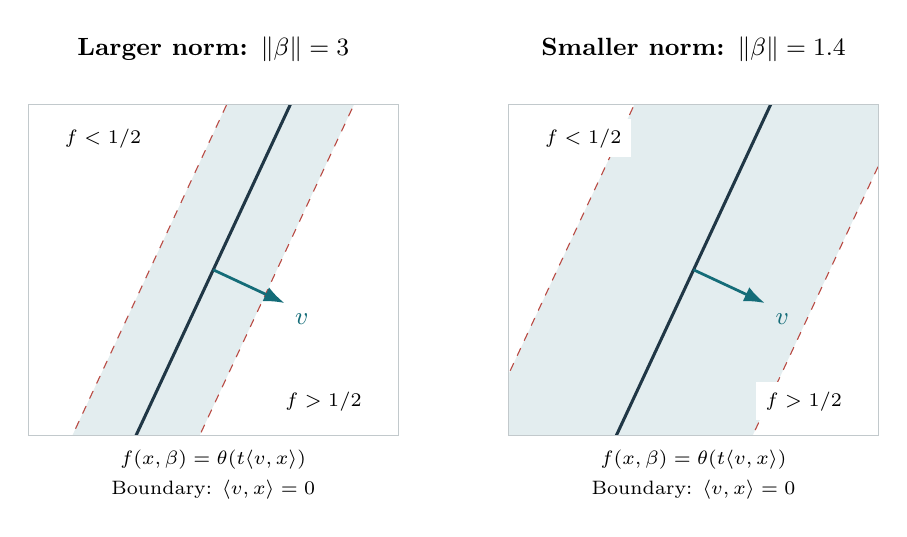
\begin{tikzpicture}[x=1cm,y=1cm]
\foreach \off/\t/\title in {0/3/Larger norm,6.1/1.4/Smaller norm}{
\begin{scope}[shift={(\off,0)}]
\node[font=\small\bfseries] at (0,2.8) {\title: $\|\beta\|=\t$};
\begin{scope}
\clip (-2.35,-2.1) rectangle(2.35,2.1);
\begin{scope}[rotate=-25]
\fill[accent!12] ({-ln(9)/\t},-3.2) rectangle({ln(9)/\t},3.2);
\draw[signalred,dashed] ({-ln(9)/\t},-3.2)--({-ln(9)/\t},3.2);
\draw[signalred,dashed] ({ln(9)/\t},-3.2)--({ln(9)/\t},3.2);
\draw[ink,line width=1.1pt] (0,-3.2)--(0,3.2);
\draw[->,accent,line width=1pt] (0,0)--(1,0) node[below right] {$v$};
\end{scope}
\end{scope}
\draw[muted!40] (-2.35,-2.1) rectangle (2.35,2.1);
\node[font=\scriptsize,fill=white] at (-1.4,1.67) {$f<1/2$};
\node[font=\scriptsize,fill=white] at (1.4,-1.67) {$f>1/2$};
\node[align=center,font=\scriptsize] at (0,-2.6) {$f(x,\beta)=\theta(t\langle v,x\rangle)$\\[3pt]Boundary: $\langle v,x\rangle=0$};
\end{scope}}
\end{tikzpicture}
\end{document}
